\subsection{Исследование системы управления с \\ пропорционально-дифференциальным регулятором} \label{title:PDR}
Составим систему
дифференциальных уравнений в операторной форме  для математического описания системы с пропорционально-дифференциальным регулятором 
относительно отклонения $x$.
\begin{figure}[!h]\centering
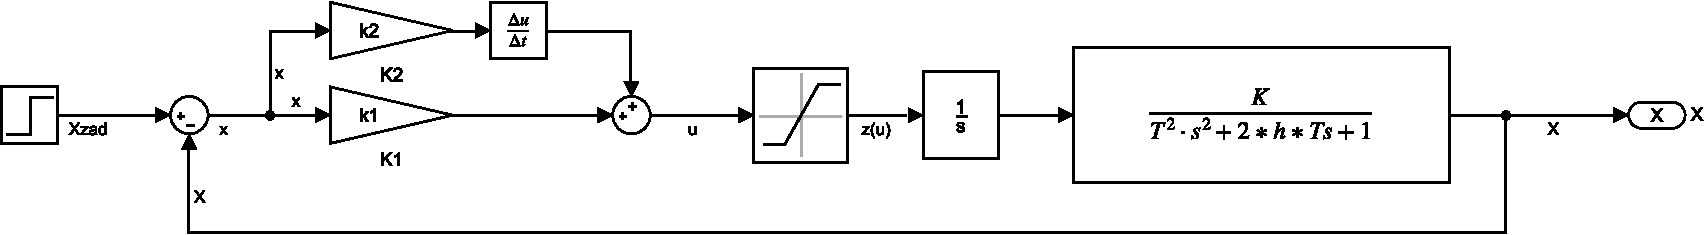
\includegraphics[width=1.0\linewidth]{images/sim_PD}
\caption{СС замкнутой системы с пропорционально-дифференциальным регулятором.}\label{fig:sim_PD}
\end{figure}
По СС замкнутой системы на рис.\ref{fig:sim_PD} составим уравнения \eqref{eq:con_PD}.
\begin{equation}
    \begin{aligned} \label{eq:con_PD}
       x&=X_{zad}-X & X&=\cfrac{3\,z(u)}{Q(p)}\\
       Q(p)&=p\,\left(81\,p^2+108\,p+1\right)&Q(p)\,x&=Q(p)\,X_{zad}-3z(u)\\
    \end{aligned}
\end{equation}
Исследуем собственные свойства системы, т.е. считаем $X_{zad}=0$.
 Учтём, что мы имеем пропорционально-дифференциальныq регулятор, т.е. $u\hm{=}k_1\,x\hm{+}k_2\,\cfrac{d\,x}{d\,t}$, получаем уравнение
 \eqref{eq:con_PD1}
.
\begin{equation} \label{eq:con_PD1}
Q(p)\,x=-3\,z(k_1\,x+k_2\,\cfrac{d\,x}{d\,t})
\end{equation}
Далее раскроем функцию $z(u)$ и получим систему \eqref{eq:con_PD2}.
\begin{equation}
    \left\{
    \begin{aligned} \label{eq:con_PD2}
       p\,\left(81\,p^2+108\,p+1\right)\,x&=-3\,\left(k_1\,+k_2\,p\right)\,x&&, \text{ если}|u|\le 0.6\\
       p\,\left(81\,p^2+108\,p+1\right)\,x&=-1.8\,\mathrm{sign}\left(u\right)&&, \text{ если}|u|> 0.6\\
    \end{aligned}
    \right.
\end{equation}
Отсюда ХП замкнутой системы при $u\le0.6$ \eqref{eq:HP_PD}.
\begin{equation} \label{eq:HP_PD}
D(p)=\left(81\,p^3+108\,p^2+p\,\left(1+3\,k_2\right)+3\,k_1\right)
\end{equation}
При $|u|>0.6$ линейная обратная связь отсутствует и движение в ней определяется свойствами управляемого объекта, при условии, что на его вход подаётся постоянное по значению воздействие. При $|u|\le0.6$ движение описывается линейным дифференциальным уравнением.

Определение предельного значения по критерию Гурвица:

$a_0=81,a_1=108,a_2=1+3\,k_2,a_3=3\,k_1$
\begin{equation} \label{eq:key5}
a_1\.a_2-a_0\,a_3\ge0
\end{equation}
\begin{equation} \label{eq:sys_ust_PD}
k_2\ge\cfrac{3\,k_{1}}{4}-\cfrac{1}{3} \text{ --- для асимптотической устойчивости.}
\end{equation}
\begin{equation} \label{eq:as_ust_PD}
k_{2\text{г.у.}}(k_1)=\cfrac{3\,k_{1}}{4}-\cfrac{1}{3}\text{ --- граница устойчивости.} 
\end{equation}

Оценим ПХ регулируемой переменной при различных значениях $k_1,k_2$ для устойчивых режимов на рис.\ref{fig:PD_sys}. 
 Несколько значений записаны в табл.\ref{tab:k1k2PD}, а алгоритм их расчёта записан в табл.\ref{tab:k1k2PDcalc}.

\begin{table}[!h] \centering
    \caption{Алгоритм расчёта значений $k_1,k_2$} \label{tab:k1k2PDcalc}
    \begin{tabular}{|c|c|c|c|c|c|}
        \hline
        $k_1$& $44$& $44$& $44$& $44$& $44$ \\ \hline
        $k_2$& $k_{2\text{г.у.}}(44)\cdot1$& $k_{2\text{г.у.}}(44)\cdot5$& $k_{2\text{г.у.}}(44)\cdot11$& $k_{2\text{г.у.}}(44)\cdot12$& $k_{2\text{г.у.}}(44)\cdot15$ \\ \hline
    \end{tabular}
\end{table}

\begin{table}[!h] \centering
    \caption{Различные значения $k_1,k_2$} \label{tab:k1k2PD}
    \begin{tabular}{|c|c|c|c|c|c|}
        \hline
        $k_1$& $44$& $44$& $44$& $44$& $44$ \\ \hline
        $k_2$& $33$& $165$& $363$& $396$& $495$ \\ \hline
    \end{tabular}
\end{table}
По графику видно, что для устойчивых режимов движения можно подбирать коэффициенты так, чтобы увеличить быстродействие системы,однако существенно изменить его невозможно. Уже при $k_1=44$ время регулирования уменьшается незначительно и составляет примерно $23$ сек, хотя и этот результат намного лучше, чем время регулирования, полученное c пропорциональным регулятором в пункте \ref{title:PR}. При анализе табл.\ref{tab:k1k2PDcalc} и рис.\ref{fig:PD_sys},видно, что с ростом множителя при $k_{2\text{г.у.}}(k_1)$ ,т.е. с ростом $k_2$, колебательность уменьшается. Таким образом $k_1$ --- коэффициент пропорциональногозвена, влияет на скорость нарастания выходной величины, а $k_2$ --- коэффициент дифференцирующего звена, влияет на колебательность системы.
\begin{figure}[!h]\centering
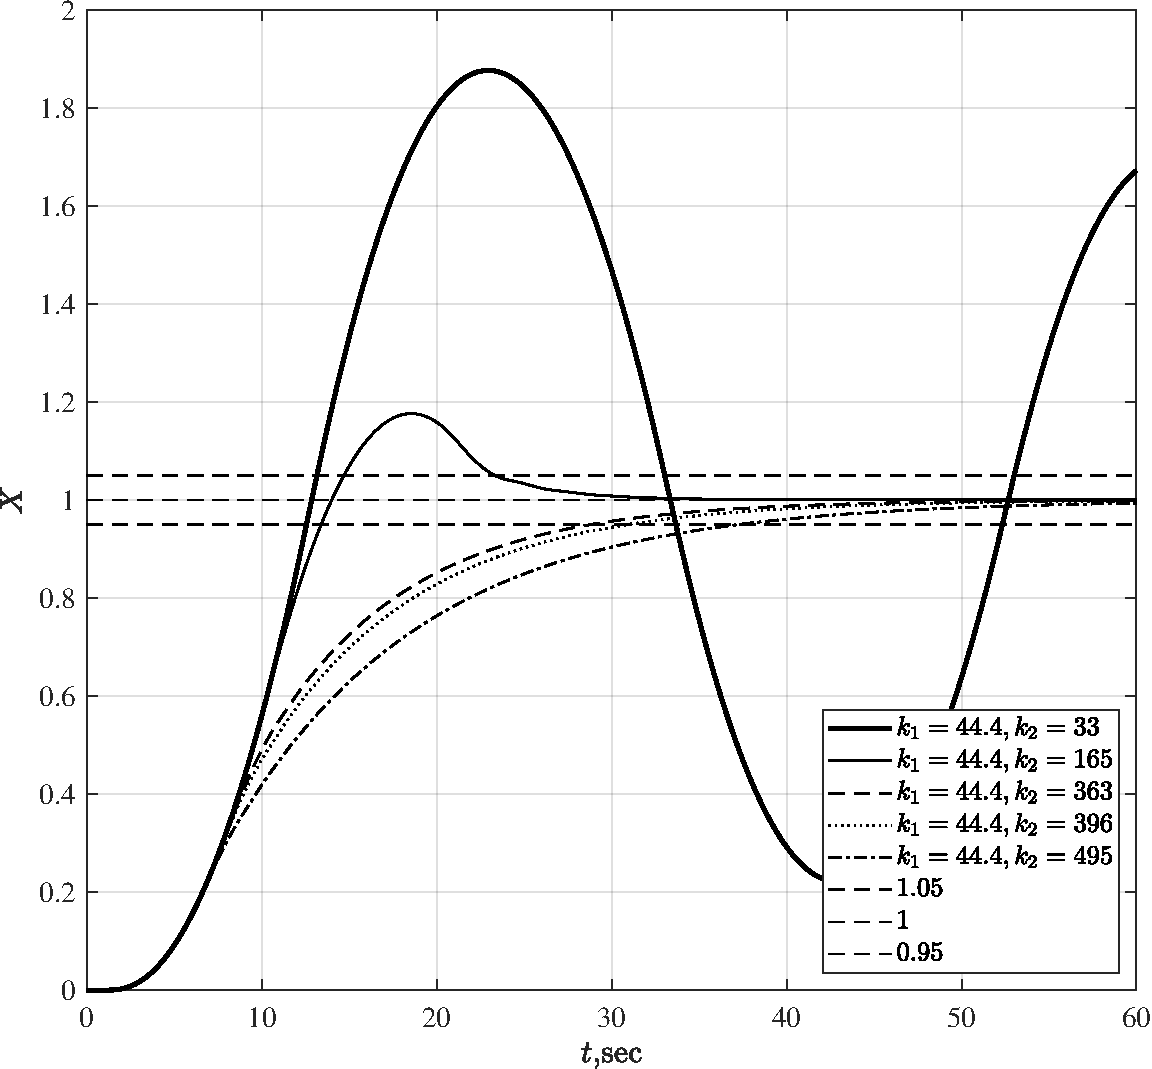
\includegraphics[width=1.0\linewidth]{images/PD_sys}
\caption{ Графики изменения выходной переменной $X$ для разных $k_1,k_2$.}\label{fig:PD_sys}
\end{figure}
